\section{Every hard-prime witness lies in the eight-sheet domain}
\label{sec:hard-prime-domain}

The earlier exterior-state theorem can be strengthened without an exterior
channel hypothesis.  Throughout this section \(p\) is a positive prime with
\(p\equiv1\pmod {12}\), and

\begin{equation}
 \frac4p=\frac1x+\frac1y+\frac1z,
 \qquad x,y,z\in\mathbb Z_{>0}.                       \tag{EZ49}
\end{equation}

\begin{theorem}[Distinctness of every hard-prime witness]
\label{thm:hard-prime-distinct}
The four integers \(p,x,y,z\) in EZ49 are pairwise distinct.  Consequently
the normalized literal-root quartic EZ6 has nonzero discriminant, and its
Fable inverse has eight distinct signed states.
\end{theorem}

\begin{proof}
If one denominator equals \(p\), relabel it as \(x=p\).  Then

\[
 \frac3p=\frac1y+\frac1z,
 \qquad (3y-p)(3z-p)=p^2.
\]

Positivity of the reciprocal equation gives \(y,z>p/3\), so both factors are
positive integers.  Since \(p\) is prime, each factor belongs to
\(\{1,p,p^2\}\).  Every element of this set is \(1\pmod3\), because
\(p\equiv1\pmod3\), whereas \(3y-p\equiv2\pmod3\).  This is impossible.

If two denominators coincide, relabel them as \(x=y=a\).  Positivity gives
\(a>p/2\).  Put \(d=2a-p>0\).  Exact rearrangement of EZ49 gives

\[
 4dz=p(d+p),
\]

so \(d\mid p^2\).  The three possibilities \(d=1,p,p^2\) give, respectively,

\[
 z=\frac{p(p+1)}4,\qquad z=\frac p2,\qquad z=\frac{p+1}4.
\]

None is integral when \(p\equiv1\pmod4\).  Symmetry excludes every collision
of these two types.  Thus all four literal roots are distinct.  At every
simple root \(t\), the equation \(\xi^2h_u'(t)=1\) has two nonzero solutions;
the root and the sign distinguish the resulting eight source points.
\end{proof}

\begin{theorem}[Fixed-input separation and inverse bounds]
\label{thm:hard-prime-bounds}
Relabel the denominators so that \(x<y<z\), and define

\begin{equation}
 R=4x-p,\qquad S_R=px=\frac{p(p+R)}4,\qquad
 s_p=\frac{p(p+3)}4,\qquad
 B_p=p+s_p(s_p+1).                                   \tag{EZ50}
\end{equation}

Then

\begin{equation}
 \frac p4<x<\frac{3p}4,\qquad 3\le R\le2p-3,          \tag{EZ51}
\end{equation}

and

\begin{equation}
 (Ry-S_R)(Rz-S_R)=S_R^2,\qquad
 z\le\frac{s_p(s_p+1)}3,\qquad
 S=p+x+y+z\le B_p.                                   \tag{EZ52}
\end{equation}

For \(t_1,t_2,t_3,t_4=p,x,y,z\),

\begin{equation}
 \boxed{\Disc(h_u)
 =S^{-6}\prod_{j<k}(t_j-t_k)^2
 \ge\frac{144}{B_p^6}.}                              \tag{EZ53}
\end{equation}

At every selected root \(t_j\),

\begin{equation}
 \frac2S\le |h_u'(t_j)|\le S^2,\qquad
 \frac1S\le|\xi_j|\le\sqrt{\frac S2}.                \tag{EZ54}
\end{equation}

The complete inverse point \(q_j=(\xi_j,y_j,z_j,w_j)\), with the coordinates
of EZ13 retained, satisfies

\begin{equation}
 |y_j|\le2S,\qquad |z_j|\le6S^2,\qquad |w_j|\le41S^3. \tag{EZ55}
\end{equation}

If \(G\) is any specified positive-definite Hermitian Gram matrix in these
four source coordinates and \(\|G\|_2\) is its spectral norm, then

\begin{equation}
 \boxed{
 \|q_j\|_G^2\le\|G\|_2
 \left(\frac S2+4S^2+36S^4+1681S^6\right).}          \tag{EZ56}
\end{equation}
Every right-hand side can be made a function of \(p\) alone by replacing
\(S\) with \(B_p\); the lower bounds become \(2/B_p\) and \(1/B_p\).
\end{theorem}

\begin{proof}
Since \(x\) is the smallest denominator,
\(1/x<4/p<3/x\), which proves the first inequalities in EZ51.  Because
\(p\equiv1\pmod4\), the positive integer \(R=4x-p\) is \(3\pmod4\).
The strict upper bound on \(x\) then gives \(3\le R\le2p-3\).

The remaining two reciprocals satisfy

\[
 \frac1y+\frac1z=\frac{R}{S_R}.
\]

Multiplication gives the first identity in EZ52.  Both factors on its left
are positive: each of \(1/y\) and \(1/z\) is strictly smaller than their sum
\(R/S_R\).  Hence \(Rz-S_R\le S_R^2\), and

\[
 z\le\frac{S_R(S_R+1)}R.
\]

The following subtraction is exact:

\[
 \frac{S_R(S_R+1)}R-\frac{s_p(s_p+1)}3
 =\frac{p^2(R-3)}{16}
   \left(1-\frac{p^2+4}{3R}\right).
\]

It is nonpositive on EZ51 because

\[
 p^2+4-3R\ge p^2+4-3(2p-3)=(p-3)^2+4>0.
\]

This proves the bound on \(z\).  Since \(x+y+z\le3z\), it also proves
\(S\le B_p\).

For four ordered distinct integers, their six positive pairwise gaps are at
least \(1,1,1,2,2,3\); their product is at least \(12\).  The normalized
leading coefficient is \(-S^{-1}\), so the quartic discriminant is the first
expression in EZ53 and the asserted lower bound follows.

At a root,

\[
 h_u'(t_j)=-S^{-1}\prod_{\ell\ne j}(t_j-t_\ell).
\]

The three signed differences are distinct nonzero integers, and their
absolute product is at least \(2\).  Each absolute difference is smaller
than \(S\).  This proves the derivative bounds.  Taking absolute values in
\(\xi_j^2h_u'(t_j)=1\) proves the bounds on \(\xi_j\).

Put \(v=|\xi_j|^{-1}\le S\) and \(t=t_j\le S\).  The literal coefficient
bounds are \(|A|=S^{-1}\) and \(|B|<S\).  Applying them term by term to EZ13
gives

\[
 |y_j|\le t+v\le2S,
\]

\[
 |z_j|\le |A|v^3+2tv+3v^2\le6S^2,
\]

and

\[
 |w_j|\le7t^2v+(|B|+17t+|A|t^2)v^2+13v^3+2|A|v^4
 \le41S^3.
\]

Finally \(q_j^*Gq_j\le\|G\|_2\|q_j\|_2^2\), and EZ54--55 give EZ56.
\end{proof}

The preceding theorem is a compactness statement only after \(p\) has been
fixed.  Its bounds grow with \(p\), and it neither proves that a witness exists
nor bounds the separate odd receiving divisor away from zero.

\section{The fixed-input signed cover}
\label{sec:fixed-input-cover}

Fix \(p\in\mathbb C^\times\).  On the coefficient hypersurface, retain both
the intrinsic-root relation \(p=-5D/C\) and EZ9.  On \(ACD\ne0\), these two
relations are equivalent to

\begin{equation}
 D=-\frac{pC}{5},\qquad
 B=-Ap^2-p-\frac{4C}{5p}.                             \tag{EZ57}
\end{equation}

Substitution gives

\begin{equation}
 h_u(r)=(r-p)g_p(r),\qquad
 g_p(r)=Ar^3+(1+Ap)r^2-\frac{4C}{5p}r+\frac C5,       \tag{EZ58}
\end{equation}

and

\begin{equation}
 d_p=g_p(p)=2Ap^3+p^2-\frac{3C}{5},\qquad
 \Disc(h_u)=d_p^2\Disc(g_p).                         \tag{EZ59}
\end{equation}

Let

\[
 \mathcal B_p=\{(A,C):A C d_p\Disc(g_p)\ne0\},
\]

and let \(\mathcal R_p\) be its coordinate ring.  The factor \(C\) is retained
because this is the intrinsic-prime ES chart.  The exact squarefreeness
boundary at fixed \(p\ne0\) is \(A d_p\Disc(g_p)=0\).

\begin{theorem}[Rank \(2+6\) decomposition]
\label{thm:fixed-input-split}
In \(\mathcal R_p[r]/(h_u)\),

\begin{equation}
 e_p(r)=\frac{g_p(r)}{d_p}                            \tag{EZ60}
\end{equation}

is the idempotent equal to one at the marked root \(p\) and zero at the three
denominator roots.  The signed inverse algebra splits as

\begin{equation}
\boxed{
\begin{aligned}
 \mathcal S_p\simeq{}&
 \mathcal R_p[\xi]/(\xi^2d_p-1)\\
 &\times
 \left(\mathcal R_p[r]/(g_p)\right)[\xi]
 \big/\left(\xi^2(r-p)g_p'(r)-1\right).
\end{aligned}}                                      \tag{EZ61}
\end{equation}

The two factors have ranks two and six over \(\mathcal R_p\).
\end{theorem}

\begin{proof}
Substituting the first identity of EZ57 into EZ9 gives

\[
 -C^3(5Ap^3+5p^2+5pB+4C)=0,
\]

which gives the second identity of EZ57 because \(pC\ne0\).  Direct
multiplication proves EZ58.  The resultant product formula gives EZ59.
Chinese remaindering by the coprime factors \(r-p\) and \(g_p\) gives the
idempotent EZ60.  Finally

\[
 h_u'(p)=d_p,\qquad h_u'(r)=(r-p)g_p'(r)\quad\text{on }g_p(r)=0,
\]

and substituting these identities into \(\xi^2h_u'(r)=1\) proves EZ61.
\end{proof}

\begin{theorem}[Order-\(48\) monodromy and exact deck group]
\label{thm:fixed-input-monodromy}
Label the marked root by \(0\) and the denominator roots by \(1,2,3\).  The
monodromy image on the eight signed states over \(\mathcal B_p\) is

\begin{equation}
 \boxed{
 G_p=\left\{(\sigma,\pi)\in\{\pm1\}^4\rtimes S_4:
 \pi(0)=0,
 \ \prod_{j=0}^3\sigma_j=\operatorname{sgn}(\pi)\right\},}
 \qquad |G_p|=48.                                    \tag{EZ62}
\end{equation}

The deck group of the disconnected rank-\(2+6\) cover is

\begin{equation}
 \boxed{\operatorname{Deck}(\mathcal S_p/\mathcal B_p)
 \simeq C_2\times C_2.}                              \tag{EZ63}
\end{equation}
\end{theorem}

\begin{proof}
Let \(\Delta=\prod_{j<k}(t_k-t_j)\).  Since

\[
 \prod_jh_u'(t_j)=A^4\Delta^2,
\]

the retained signed invariant

\[
 \chi=A^2\Delta\prod_j\xi_j\in\{1,-1\}
\]

is locally constant.  Continuation by \((\sigma,\pi)\) therefore forces
\(\prod_j\sigma_j=\operatorname{sgn}(\pi)\).  The marked root cannot move,
which proves the upper bound in EZ62.

Define the ordered denominator space \(X_p\) by choosing \((x,y)\in\mathbb
C^2\), putting

\begin{equation}
 z=\frac{pxy}{4xy-p(x+y)},                            \tag{EZ64}
\end{equation}

and deleting the loci on which a denominator is zero, two of
\(p,x,y,z\) collide, the denominator in EZ64 vanishes, or
\(S=p+x+y+z\) vanishes.  This is the complement of finitely many complex
algebraic curves in \(\mathbb C^2\), and it is nonempty.  It is also path
connected.  Given two retained points, the complex affine line through them
cannot be contained in any deleted curve, because both endpoints lie outside
that curve.  It therefore meets each deleted algebraic curve in finitely many
points.  A complex line with finitely many points removed is path connected,
so the two retained points are joined inside \(X_p\).

There is an exact coefficient map

\[
 q_p:X_p\longrightarrow\mathcal B_p,
 \qquad
 q_p(x,y)=\left(-\frac1{p+x+y+z},
                 \frac{5xyz}{p+x+y+z}\right)=(A,C).
\]

It is invariant under all six reorderings of \((x,y,z)\).  The reciprocal
equation and the two displayed coefficients give the literal identity

\[
 A\prod_{t\in\{p,x,y,z\}}(r-t)=(r-p)g_p(r).
\]

The deletions in the definition of \(X_p\) then give
\(ACd_p\Disc(g_p)\ne0\), so \(q_p\) lands in \(\mathcal B_p\).
Conversely, for
\((A,C)\in\mathcal B_p\), the unordered denominator triple is exactly the
root set of

\[
 \frac{g_p(r)}A
 =r^3+\left(p+\frac1A\right)r^2
   -\frac{4C}{5pA}r+\frac{C}{5A}.
\]

Thus its elementary symmetric functions are

\[
 x+y+z=-p-\frac1A,\qquad
 xy+xz+yz=-\frac{4C}{5pA},\qquad
 xyz=-\frac{C}{5A}.
\]

They obey \(p(xy+xz+yz)=4xyz\), which is precisely the reciprocal
Erd\H{o}s--Straus equation and gives EZ64.  The factors defining
\(\mathcal B_p\) say exactly that these roots are nonzero, mutually distinct,
different from \(p\), and have \(S\ne0\).  Hence every fibre of \(q_p\) is
the free six-element ordering orbit, and the elementary-symmetric inverse
proves the exact quotient

\[
 X_p/S_3\;\xrightarrow{\ \sim\ }\;\mathcal B_p.
\]

Since \(X_p\) is connected, this finite \(S_3\)-cover has unsigned monodromy
equal to all of \(S_3\).

The sign subgroup is realized by two exact local families.  First put

\[
 x=p(2+w),\qquad y=p(2-w),\qquad
 z=p\frac{4-w^2}{12-4w^2}.
\]

For \(0<|w|\le1/10\), only \(x=y\) occurs inside the puncture.  The two
coefficient and derivative factors are

\[
 A=-\frac{4(w^2-3)}{p(21w^2-64)},\qquad
 C=-\frac{5p^2(w-2)^2(w+2)^2}{21w^2-64},
\]

\[
 h_u'(p)=
 \frac{p^2(w-1)(w+1)(3w^2-8)}{21w^2-64},
\]

\[
 h_u'(x)=
 -\frac{2p^2w(w+1)(w+2)(4w^2-w-10)}{21w^2-64},
\]

\[
 h_u'(y)=
 \frac{2p^2w(w-2)(w-1)(4w^2+w-10)}{21w^2-64}.
\]

\[
 h_u'(z)=
 -\frac{p^2(w-2)(w+2)(3w^2-8)
 (4w^2-w-10)(4w^2+w-10)}
 {16(w^2-3)^2(21w^2-64)}.
\]

On \(|w|\le1/10\), the estimates
\(|21w^2|<64\), \(|3w^2|<8\), and
\(|4w^2\mathbin{\pm}w|<10\), together with
\(|w|<1<2\), prove that every displayed base factor and every derivative
factor other than the single \(w\)-factor in \(h_u'(x),h_u'(y)\) is nonzero.
Thus the path stays in \(\mathcal B_p\) away from its central collision.  A
half-circle exchanges \(x,y\); its square fixes the labels and flips exactly
their two square-root signs.

Next put

\[
 x=p(1+w),\qquad y=\frac{2p}{5},\qquad
 z=\frac{2p(1+w)}{1+3w}.
\]

For \(0<|w|\le1/100\), only \(p=x\) occurs inside the puncture, and

\[
 A=-\frac{5(3w+1)}{p(15w^2+51w+22)},\qquad
 C=\frac{20p^2(w+1)^2}{15w^2+51w+22},
\]

\[
 h_u'(p)=\frac{3p^2w(w-1)}{15w^2+51w+22},
\]

\[
 h_u'(x)=
 -\frac{p^2w(w+1)(3w-1)(5w+3)}{15w^2+51w+22}.
\]

\[
 h_u'(y)=
 \frac{12p^2(w+2)(5w+3)}{25(15w^2+51w+22)},
\]

\[
 h_u'(z)=
 -\frac{4p^2(w-1)(w+1)(w+2)(3w-1)}
 {(3w+1)^2(15w^2+51w+22)}.
\]

For \(|w|\le1/100\),
\(|15w^2+51w|<22\); all remaining displayed linear factors are separated
from zero except the single \(w\)-factor in \(h_u'(p),h_u'(x)\).  Hence this
path also stays in \(\mathcal B_p\) away from its central collision.  A full circle fixes every root
label and flips exactly the signs over \(p,x\).  Denominator pair flips span
the even-sign plane on the three denominator labels; adjoining this
prime--denominator flip spans all eight even sign vectors.  With the six
denominator permutations, the realized image has \(8\cdot6=48\) elements and
attains the upper bound.

The two connected sheet-orbits have sizes two and six.  On the six
denominator sheets, the induced action is the full signed permutation group
\(C_2^3\rtimes S_3\), whose centralizer is generated by simultaneous
denominator sign reversal.  The prime-pair centralizer is \(C_2\).  The two
deck maps can be written

\[
 \xi\longmapsto(1-2e_p)\xi,\qquad \xi\longmapsto-\xi.
\]

They independently reverse the prime pair and the denominator sheets, and
their products exhaust the centralizer.  This proves EZ63.
\end{proof}

\begin{corollary}[Correct order-\(48\) orbit metric]
\label{cor:fixed-input-metric}
In even/odd coordinates for each signed root pair, the eight-dimensional
representation is

\begin{equation}
 \mathbf1^{\oplus2}\oplus V_2\oplus\chi_{\det}\oplus V_3,       \tag{EZ65}
\end{equation}

where \(V_2\) is the standard two-dimensional \(S_3\)-module,
\(V_3\) is the three-dimensional signed-permutation module, and

\[
 \chi_{\det}(\sigma,\pi)
 =\operatorname{sgn}(\pi)\prod_{i=1}^3\sigma_i=\sigma_0.
\]

Let \(E=[e_p,E_d]\) and \(O=[o_p,O_d]\) be the original even and odd source
columns, and let \(G\) be the specified receiving form.  Averaging the pulled
back Gram matrix over \(G_p\), in the corresponding orthonormal decomposition,
gives

\begin{equation}
 \boxed{H_{\rm triv}\oplus\lambda_2I_2\oplus\lambda_p
 \oplus\lambda_3I_3,}                                \tag{EZ66}
\end{equation}

where

\[
 H_{\rm triv}=
 \begin{bmatrix}e_p&E_d\mathbf1/\sqrt3\end{bmatrix}^{*}G
 \begin{bmatrix}e_p&E_d\mathbf1/\sqrt3\end{bmatrix},
\]

\[
 \lambda_2=\frac12\operatorname{tr}(P_2E_d^*GE_d),
 \quad P_2=I_3-\frac13\mathbf1\mathbf1^*,
 \quad\lambda_p=o_p^*Go_p,
 \quad\lambda_3=\frac13\operatorname{tr}(O_d^*GO_d).
\]

In particular, the mutual Gram term between the prime-even state and the
denominator-even sum survives; the two-dimensional block cannot be replaced
by two unrelated scalars.
\end{corollary}

\begin{proof}
The even denominator permutation module is
\(\mathbf1\oplus V_2\), while the prime-even line is another trivial module.
The prime-odd line transforms by \(\chi_{\det}\), and the three denominator-odd
coordinates form \(V_3\).  Averaging kills maps between inequivalent
summands, retains the full Gram form on the two equivalent trivial copies,
and gives the normalized traces on the irreducible \(V_2,V_3\) blocks.  The
one-dimensional \(\chi_{\det}\) block is \(o_p^*Go_p\).  These are exactly the
four blocks in EZ66.
\end{proof}

\begin{figure}[htbp]
\centering
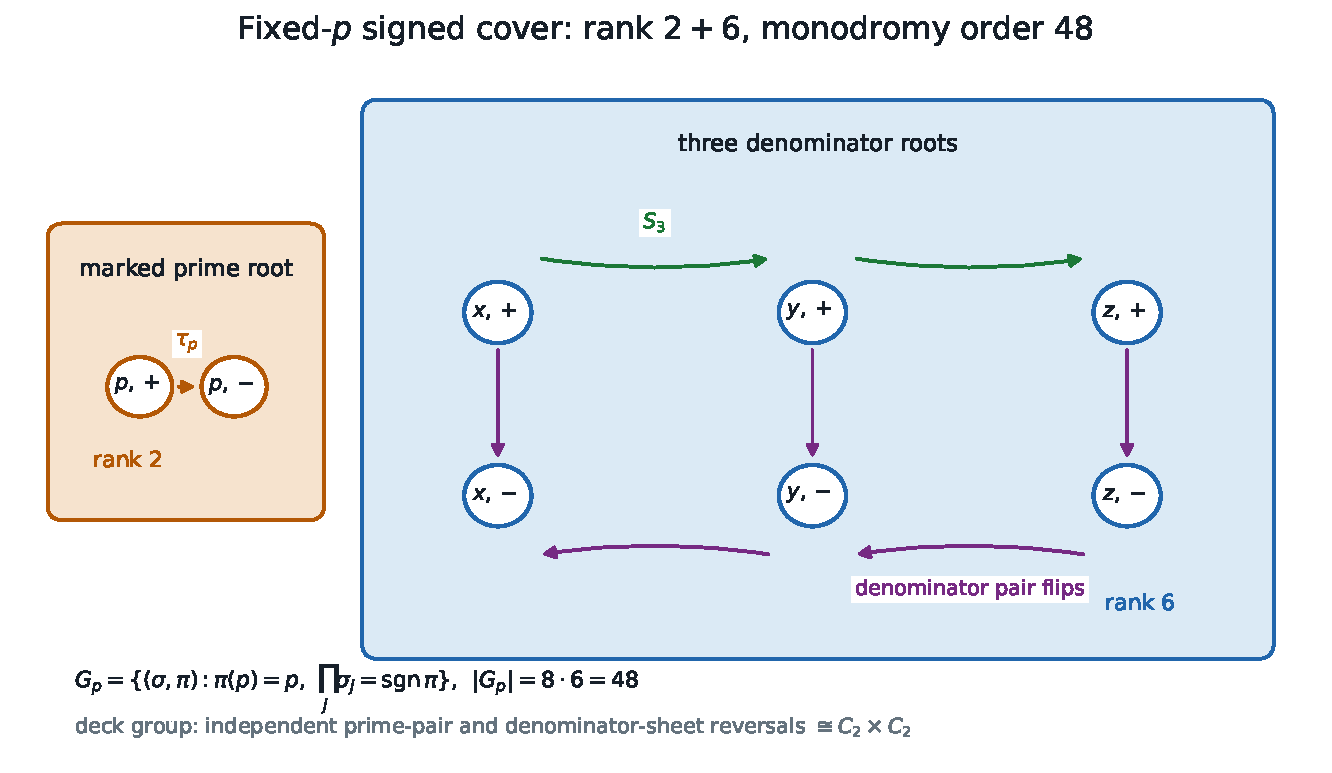
\includegraphics[width=.94\textwidth]{figures/fixed-input-cover-decomposition.pdf}
\caption{The proved fixed-input decomposition.  The marked prime produces a
rank-two component and the three denominator roots a rank-six component.
Denominator permutations, denominator pair flips, and one
prime--denominator flip generate the order-\(48\) monodromy; the two displayed
deck reversals commute with it.  This is a sheet-action diagram, not a metric
embedding.  Reproduce it with
\texttt{tools/generate\_20260920\_illustrations.py}; exact group enumeration
is in \texttt{verify\_fixed\_input\_boundary.py}.}
\label{fig:fixed-input-cover}
\end{figure}

\section{Finite completion of the inverse-derivative boundary}
\label{sec:finite-completion}

Work over

\[
 \mathcal R_0=\mathbb C[A,A^{-1},B,C,D],\qquad
 \mathcal E=\mathcal R_0[r]/(h_u).
\]

Introduce the reciprocal signed coordinate \(\eta=\xi^{-1}\) and define

\begin{equation}
 \boxed{\widehat{\mathcal S}
 =\mathcal E[\eta]/(\eta^2-h_u'(r)).}                 \tag{EZ67}
\end{equation}

\begin{theorem}[Finite flat rank-eight completion]
\label{thm:finite-completion}
The algebra EZ67 is free of rank eight over \(\mathcal R_0\), with basis

\begin{equation}
 1,r,r^2,r^3,\eta,\eta r,\eta r^2,\eta r^3.           \tag{EZ68}
\end{equation}

It recovers the original signed inverse exactly on \(\eta\ne0\):

\begin{equation}
 \boxed{
 \mathcal E[\xi]/(\xi^2h_u'-1)
 \simeq\widehat{\mathcal S}[\eta^{-1}],\qquad
 \eta=\xi h_u'=\xi^{-1},\quad \xi=\eta^{-1}.}         \tag{EZ69}
\end{equation}

Thus its spectrum is finite flat of degree eight and proper over
\(\operatorname{Spec}\mathcal R_0\).  Its ramification Jacobian in the
\((r,\eta)\) variables is

\begin{equation}
 \det
 \begin{pmatrix}h_u'(r)&0\\-h_u''(r)&2\eta\end{pmatrix}
 =2\eta h_u'(r)=2\eta^3.                              \tag{EZ70}
\end{equation}
\end{theorem}

\begin{proof}
Because \(A\) is a unit, \(A^{-1}h_u\) is monic of degree four; hence
\(\mathcal E\) is free of rank four.  The relation in EZ67 is monic of degree
two in \(\eta\), which proves EZ68.  Inverting \(\eta\) and setting
\(\xi=\eta^{-1}\) gives \(\xi^2h_u'=1\).  Conversely, in the original signed
algebra, \(\eta=\xi h_u'\) is the inverse of \(\xi\) and satisfies
\(\eta^2=h_u'\).  This proves EZ69.  A finite morphism is proper
\cite{StacksFinite}.  Direct differentiation gives EZ70; away from
\(\eta=0\), its determinant is a unit, agreeing with the standard
derivative-unit criterion for an étale algebra \cite{StacksEtale}.
\end{proof}

The completion is over \(A\ne0\).  It does not repair the independent
infinity-chart boundary \(A=0\).

\begin{proposition}[The original meromorphic pole is retained]
\label{prop:retained-pole}
In the completed coordinates, the original inverse point is

\begin{equation}
 q=\begin{pmatrix}
 \eta^{-1}\\
 -r-\ii\eta\\
 A\eta^3+2r\eta+3\ii\eta^2\\
 7\ii r^2\eta+(B-17r+Ar^2)\eta^2-13\ii\eta^3-2A\eta^4
 \end{pmatrix}.                                      \tag{EZ71}
\end{equation}

Let a path approach a fixed finite coefficient target of
\(\operatorname{Spec}\mathcal R_0\), with \(\eta\to0\); equivalently the
coefficients and \(r\) remain bounded and \(A\) stays nonzero.  For any fixed
injective receiving map \(F\), with positive target form \(Q\) and
\(G=F^*QF\),

\begin{equation}
 \boxed{|\eta|\,\|Fq\|_Q\longrightarrow\sqrt{G_{11}}>0.}       \tag{EZ72}
\end{equation}
\end{proposition}

\begin{proof}
Formula EZ71 is EZ13 after substituting \(\xi=\eta^{-1}\), with every term
retained.  Under the stated finite-target hypothesis,
\(\eta q\to(1,0,0,0)^{\mathsf T}\).  Taking the norm induced by \(G\) gives
EZ72.  Thus the finite algebra adds the missing boundary state but does not
turn the original meromorphic norm pole into a bounded point.
\end{proof}

\begin{theorem}[Exact nonreduced fibre at a multiple root]
\label{thm:nilpotent-fibre}
Suppose

\[
 h_u(r)=(r-r_0)^m g(r),\qquad g(r_0)=g_0\ne0.
\]

With \(\varepsilon=r-r_0\), the completed local signed fibre is

\begin{equation}
 \boxed{
 \widehat{\mathcal S}_{r_0}
 =\mathbb C[\varepsilon,\eta]/
 (\varepsilon^m,\eta^2-mg_0\varepsilon^{m-1}),\qquad
 \dim_{\mathbb C}\widehat{\mathcal S}_{r_0}=2m.}      \tag{EZ73}
\end{equation}

For a double root,

\begin{equation}
 \varepsilon=\frac{\eta^2}{2g_0},\qquad
 \boxed{\widehat{\mathcal S}_{r_0}\simeq
 \mathbb C[\eta]/(\eta^4).}                          \tag{EZ74}
\end{equation}

Multiplication by \(\varepsilon\) has two Jordan blocks of size \(m\).
\end{theorem}

\begin{proof}
The factor \(g\) is a unit in the local root algebra, so
\((h_u)=(\varepsilon^m)\).  Modulo \(\varepsilon^m\),

\[
 h_u'(r)=mg_0\varepsilon^{m-1}.
\]

This proves the presentation in EZ73.  It is free on \(1,\eta\) over
\(\mathbb C[\varepsilon]/(\varepsilon^m)\), proving the dimension and the two
Jordan blocks.  When \(m=2\), eliminating \(\varepsilon\) gives EZ74.
\end{proof}

\begin{theorem}[Exact local ES--paired-root isomorphism]
\label{thm:local-es-rh-map}
The integral ES boundary witness

\[
 \frac45=\frac15+\frac12+\frac1{10}
\]

has

\[
 h_{\rm ES}(r)=-\frac1{22}(r-5)^2(r-2)(r-10),\qquad
 \eta_{\rm ES}^2=\frac{15}{11}\varepsilon_{\rm ES}.
\]

More generally, the rational family

\begin{equation}
 (p;x,y,z)=\left(p;p,\frac{2p}{5},2p\right)           \tag{EZ75}
\end{equation}

has a double root at \(p\) with
\(\eta_{\rm ES}^2=(3p/11)\varepsilon_{\rm ES}\).

For the auxiliary paired-root quartic

\[
 h_{\rm pair}(r)=-\frac12\left((r-\tfrac12)^2+\gamma^2\right)^2,
 \qquad r_\pm=\frac12\pm\ii\gamma,
\]

one has \(\eta_{\rm pair}^2=4\gamma^2\varepsilon_{\rm pair}\) at either
double root.  If \(p\gamma\ne0\) and

\[
 c^2=\frac{3p}{44\gamma^2},
\]

then

\begin{equation}
 \boxed{
 \eta_{\rm ES}\longmapsto c\eta_{\rm pair},\qquad
 \varepsilon_{\rm ES}\longmapsto\varepsilon_{\rm pair}}       \tag{EZ76}
\end{equation}

is an isomorphism of the two length-four local algebras.  It intertwines
centred multiplication.  On uncentred coordinates,

\[
 r_{\rm ES}\longmapsto r_{\rm pair}+(p-r_\pm).
\]

In the bases \(1,\eta,\eta^2,\eta^3\), its matrix is
\(D_c=\operatorname{diag}(1,c,c^2,c^3)\).  Therefore the pullback of a target
Hermitian form \(G_{\rm pair}\) is \(D_c^*G_{\rm pair}D_c\), whose determinant
is \(|c|^{12}\det G_{\rm pair}\).
\end{theorem}

\begin{proof}
All displayed local equations follow by evaluating the residual factor \(g\)
at the double root and applying EZ73.  In EZ75 the normalized residual value
is \(g_0=3p/22\); at \(r_\pm\) it is \(g_0=2\gamma^2\).  The defining relation
is preserved by EZ76 because

\[
 c^2(4\gamma^2)=\frac{3p}{11}.
\]

The inverse uses \(c^{-1}\).  The statements about centred and uncentred
multiplication follow from
\(r_{\rm ES}=p+\varepsilon_{\rm ES}\) and
\(r_{\rm pair}=r_\pm+\varepsilon_{\rm pair}\).  The basis matrix and metric
determinant are then direct.
\end{proof}

This is a local algebra and action morphism.  It does not identify the global
fibres, their native metrics, or a varying family of zeta zeros.  It also does
not make the nilpotent action isometric.  Indeed let

\[
 N=M_{\varepsilon}=(2g_0)^{-1}M_{\eta^2}
\]

in EZ74.  Then \(N\ne0\) and \(N^2=0\).  For every positive Hermitian form
\(G\), choose \(v\) with \(Nv=w\ne0\).  In the ordered pair \((w,v)\), the
compression of \(N^*G+GN\) has matrix

\[
 \begin{pmatrix}
 0&\|w\|_G^2\\
 \|w\|_G^2&2\operatorname{Re}\langle w,v\rangle_G
 \end{pmatrix},
\]

whose determinant is \(-\|w\|_G^4<0\).  Thus it has both signs.

\begin{figure}[htbp]
\centering
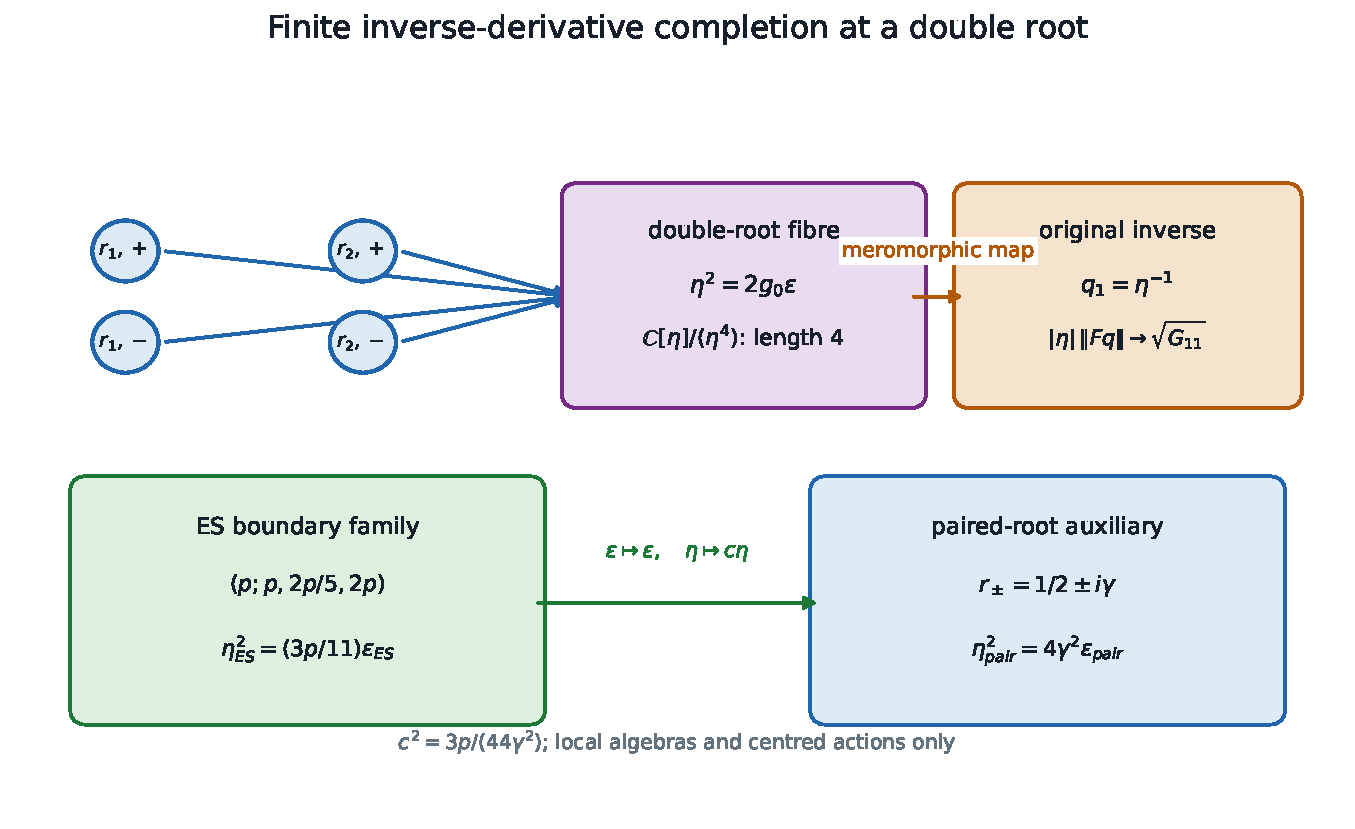
\includegraphics[width=.92\textwidth]{figures/finite-boundary-local-fibre.pdf}
\caption{The finite completion and its exact double-root fibre.  On
\(\eta\ne0\), \(\xi=\eta^{-1}\) recovers the original inverse.  At a double
root, four nearby signed states coalesce into the length-four algebra
\(\mathbb C[\eta]/(\eta^4)\), while the original first source coordinate keeps
its \(\eta^{-1}\) pole.  The lower arrow is the typed local algebra map EZ76;
it does not identify the global ES and paired-root constructions.  Reproduce
with \texttt{tools/generate\_20260920\_illustrations.py}.}
\label{fig:finite-boundary-local-fibre}
\end{figure}

\section{An invertible marked odd-moment frame}
\label{sec:odd-moment-frame}

On the ordered signed-root cover of the squarefree \(A\ne0\) coefficient
domain, retain the labels \(r_1,\ldots,r_4\) and signs
\(\xi_j^2h_u'(r_j)=1\), and define

\begin{equation}
 U=
 \begin{pmatrix}
 1&1&1&1\\
 r_1&r_2&r_3&r_4\\
 r_1^2&r_2^2&r_3^2&r_4^2\\
 r_1^3&r_2^3&r_3^3&r_4^3
 \end{pmatrix}
 \operatorname{diag}(\xi_1,\xi_2,\xi_3,\xi_4).        \tag{EZ77}
\end{equation}

\begin{theorem}[Odd-frame factorization and complete inverse]
\label{thm:odd-moment-frame}
One has

\begin{equation}
 \boxed{\det U=\frac{\chi}{A^2},\qquad\chi\in\{1,-1\}.}         \tag{EZ78}
\end{equation}

For each of the four component polynomials

\[
 1,\quad -\ii h_u',\quad A(h_u')^2+2rh_u',\quad
 \ii\bigl(7r^2h_u'-13(h_u')^2\bigr),
\]

reduce modulo \(h_u\), and let the corresponding ascending coefficient rows
in the ordered basis \(1,r,r^2,r^3\) be the rows of \(V_h\).  If \(O\) is the
original odd evaluation matrix EZ37, then

\begin{equation}
 \boxed{O=V_hU.}                                      \tag{EZ79}
\end{equation}

For \(m=U\beta\), the inverse is

\begin{equation}
\boxed{
\begin{aligned}
 \beta_j=\xi_j\bigl[&
 (C+Br_j+r_j^2+Ar_j^3)m_0\\
 &+(B+r_j+Ar_j^2)m_1
 +(1+Ar_j)m_2+Am_3\bigr].
\end{aligned}}                                      \tag{EZ80}
\end{equation}
\end{theorem}

\begin{proof}
The first matrix in EZ77 is the labelled Vandermonde matrix.  If
\(\Delta=\prod_{j<k}(r_k-r_j)\), then

\[
 \prod_jh_u'(r_j)=A^4\Delta^2,
 \qquad \left(\Delta\prod_j\xi_j\right)^2=A^{-4},
\]

which proves EZ78.  Evaluating the four reduced component polynomials at the
four roots and multiplying each column by its retained \(\xi_j\) gives EZ79.

For the inverse, synthetic division gives

\[
 \frac{h_u(r)}{r-r_j}=
 Ar^3+(1+Ar_j)r^2+(B+r_j+Ar_j^2)r
 +(C+Br_j+r_j^2+Ar_j^3).
\]

The corresponding Lagrange polynomial is this quotient divided by
\(h_u'(r_j)\).  Since
\(1/(\xi_jh_u'(r_j))=\xi_j\), applying the Lagrange coefficient functional
to \(m_0,m_1,m_2,m_3\) gives EZ80.
\end{proof}

Although \(U\) itself lives on the marked signed cover, EZ78--79 show that
the additional unmarked zero divisor of the original odd evaluation is
exactly \(\det V_h=0\), away from \(A\Disc(h_u)=0\).  At that divisor, moments
cannot be reconstructed from the already-collapsed data \(O\beta\); they must
be retained before applying \(V_h\).
